\chapter{Conclusion}
\label{chap:conclusion}

\begin{chapquote}{Roger Bacon}{``Reasoning draws a conclusion and makes us grant the conclusion, but does not make the conclusion certain, nor does it remove doubt so that the mind may rest on the intuition of truth, unless the mind discovers it by the path of experience.''}
\end{chapquote}

Glyph-based visualizations can provide real benefits when their corresponding glyphs are properly designed.
However poor glyph design will present limitations to the utility of such visualizations \cite{morris2000experimental, ward02}.
This thesis set out to explore how glyph design could be made more systematic through addition of processes that could reduce subjectivity present in a number of areas including:
the mapping process between data and visual encodings, and the arrangement of these encodings within a glyph; 
the design of glyph libraries for glyph-based visual compression; and
glyph evaluation.

As part of our exploration of the problem space, we proposed a model for systematisation in Chapter \ref{chap:strategies} that placed computational techniques and design principles as core components in the glyph design process.
While this model represented a number of strategies for systematic glyph design using computation, it was also flexible enough to consider cases where computation was not always applicable, such as the biological sequence logo and initial poetry glyph design in Chapter \ref{chap:processes}.

More importantly, through use of this model, we were able to devise strategies to investigate the research questions from Chapter \ref{chap:introduction}.
The contributions of this thesis can be summarised through answers to those questions.

\section{Contributions}
We state the contributions of this thesis through focusing on the questions from Chapter \ref{chap:introduction}.
Is glyph design amenable to systematisation by computational methods?
Can computational methods be applied to the design of glyph libraries?
Is glyph evaluation amenable to systematisation by computational methods?

% \begin{figure}[!ht]
%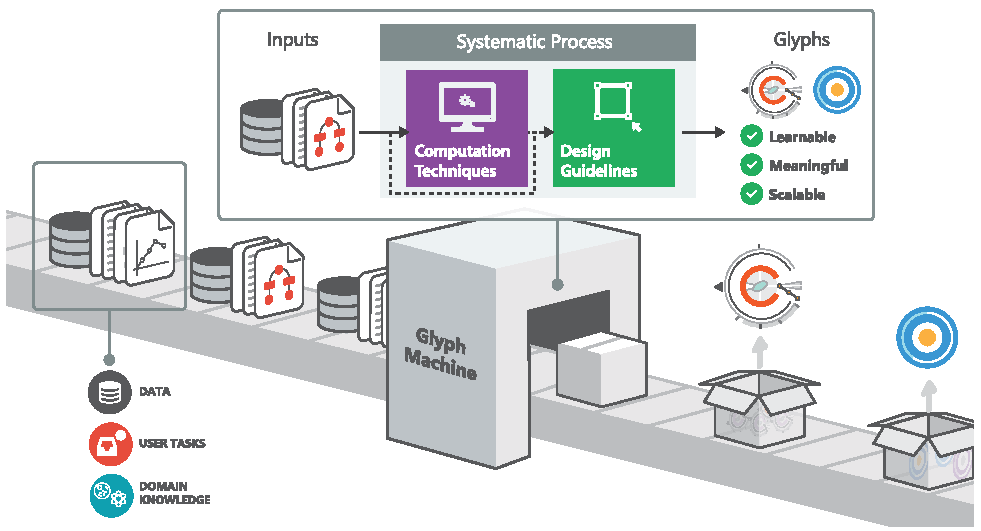
\includegraphics[width=\textwidth]{images/conclusion/systematic_design}
%\caption{Towards a systematic glyph design.}
%\label{fig:systematic_design}
%\end{figure}

\subsection{Is Glyph Design Amenable to Systematization by Computational \\Methods?}
Glyph design is bound by a number of properties of the human perception system.
In Chapter \ref{chap:related_work} we showed how it is bound by our capacity to perceive high spatial frequencies at low resolutions, by limits in how we perceive colour (hue and saturation), size, length, orientation.
Our interpretation of a visual channel is also bound by our ability to remember mappings from data to the visual channels we use to represent them.
This is why use of natural mappings, in particular metaphor, is important.

To move this knowledge to a more actionable form, we devised a number of design principles that summarise some of the more important points to consider when creating glyphs, including:
1) channel suitability;
2) natural/semantic mappings;
3) visual hierarchy (this also dictates the ``power'' of the visual channel to be used);
4) channel composition;
5) channel capacity; and
6) use of redundant encodings for important data.

While application of these principles can provide a level of systematisation, we also wished to investigate how computational approaches could remove the subjectivity in forming the visual hierarchy for instance.
A major contribution of this thesis was the creation of such a computational approach.
Our taxonomy-based approach to glyph design in Chapter \ref{chap:glyph-tax} showed for the first time how numerous components of glyph design could be informed through computation.
The taxonomy algorithm provided a hierarchical organisation that could categorise items to be represented as glyphs.
This hierarchical structure provided the basis for construction of the visual hierarchy.
The stronger visual channels, \eg, colour hue, were selected for higher levels in the taxonomy so that they could be distinguished at even low resolutions.
Less strong visual channels occupying higher spatial frequencies were mapped to lower levels in the taxonomy.

Additionally the algorithm for taxonomy generation selects for schemes that have a small number of categories (less than eight) to reduce the probability of exceeding the capacity limits of a visual channel.
The lower the number of values to be represented by a visual channel, the fewer difficulties there are in memorising and learning abstract mappings to colour or shape for example.
Moreover, a few number of values represented by a visual channel can mean a reduction in the chance of interpretation errors due to a greater distance between shapes, colours, line width, and so on.

A further example of how computational approaches can help glyph design was demonstrated in Chapter \ref{chap:processes} Section \ref{sec:poetry}.
Here, computation was used to assist the design of static and dynamic macro glyphs for poems.
We showed how structural and statistical analysis of a graph created from vowel sounds and their transitions in a poem could inform how the corresponding glyphs are composed.

\subsection{Can Computational Methods be Applied to the Design of Glyph Libraries for Visual Compression?}

Another important aspect of glyph design is deciding what to represent with glyphs to aid better visual search for events in graphs, time-series, or text data for example.
Similar to traffic signage where a number of text-based signs were converted to more iconic representations to certain events easier to see, it would be convenient to replace commonly observed patterns in a visualization with more compact glyph representations that are easier to visually search.
Meanwhile, the remainder of the visualization is left in its original form since it may be regarded as more anomalous.

A further contribution of this thesis is in the application of computational methods to enable more systematic design of glyph libraries.
Our process focuses on the use of data and statistics to suggest motifs that are candidates for visual information compression.
From these statistically informed suggestions, domain experts can filter out semantically meaningless patterns to create a semantically, and statistically informed glyph library.
To apply this process, we focused on visual compression of the workflow graphs from Chapter \ref{chap:glyph-tax}, and time series data.

First, we applied this systematic approach to graphs in Chapter \ref{chap:automacron}.
We developed a novel motif finding algorithm that considers node and edge semantics as well as topology.
This motif detection algorithm was run on nearly 11,000 studies and approximately 500,000 individual experiments to determine common structures across a representative sample of the data.
Results were presented to domain experts, and sorted on a summary score composed through use of a number of metrics.
Experts were then able to select motifs to form a glyph library for compression.
Additionally, the creation of multi-resolution glyphs (different details for different zoom factors) was automated through use of the state transition model that underpins the motif detection algorithm.

Next, in Chapter \ref{chap:timeseries} we applied this approach to time-series data.
A data-driven approach was again used where our algorithm takes a collection of time-series, statistically analyses these for common patterns, and presents the resulting patterns back to domain-experts.
Domain-experts are again in the loop to ensure that motifs are semantically relevant.

Both pieces of work have shown that a computational approach to glyph selection can work to systematise selection of motifs for glyph-based compression.
Human intervention is not removed completely, but decisions are more informed through the statistics we have introduced.

\subsection{Is Glyph Evaluation Amenable to Systematization by Computational \\Methods?}
Numerous aspects of glyphs can be evaluated, some will be domain dependent, others are more general.
For example, if glyphs are designed to encode complex cardiology data, it will be hard to assess the utility of such a glyph without input from domain experts.
 
More general types of evaluation however, such as evaluating the discriminability of a glyph, can be assessed computationally as shown in our work in Chapter \ref{chap:processes} Section \ref{sec:file_system}.
This computational approach is underpinned by a new metric to measure glyph distinguishability, named the quasi-Hamming distance (QHD).
We tested this metric by measuring the distance between visual stimuli using both human participants and an image similarity algorithm.
Our computationally-obtained distances were shown to be well correlated with user-based results.

\section{Summary and Future Research Directions}

The work presented here opens up a number of interesting research avenues around glyph-design.
While we can see that glyph design has gained more popularity in recent years \cite{Polk14, kachkaev2014, CGF:Abd2013a}, creating well designed glyphs for an effective glyph-based visualization can be difficult, especially glyphs like those given in Chapter \ref{chap:glyph-tax}.
For example, scatter plot matrices and parallel coordinate plots simply require a user to load comma-separated value (CSV) files representing the data, and the visualization is rendered.
For a glyph-based visualization we first need examples of the data to be represented, glyphs will be designed around this data, and finally, those glyphs need to be positioned in a display.
The systematic approaches presented in this thesis go some way to simplifying the design step, but more needs to be done to make the process even simpler for users, making it as easy to create effective glyph-based visualizations as it is to create parallel coordinate plots.

Future research directions should build upon the techniques presented in this work and drive towards more automatic glyph design and evaluation.
This would make glyph-based visualizations for data exploration something that any user could deploy.
The path towards such a vision lies in what I believe to be a number of future developments:
\begin{enumerate}
\item \textbf{A glyph encoder/decoder} illustrated in Figure \ref{fig:encode_decode} that would extend on this thesis to investigate both how automatised encoding of glyphs can be accomplished, and how much ``information'' could be decoded from glyphs.

\begin{figure}[t!]
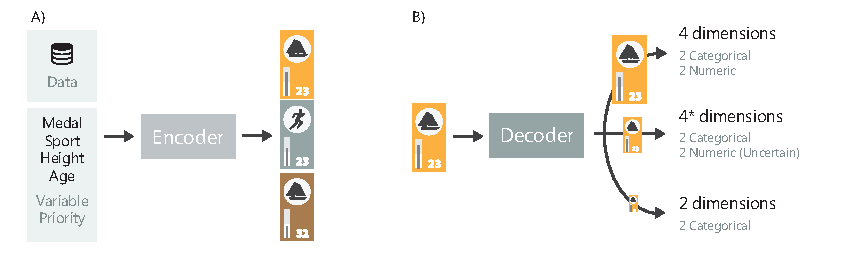
\includegraphics[width=\textwidth]{images/conclusion/encode_decode}
\caption{A) A glyph \emph{encoder} can take a set of data, with variable priority and automatically create glyphs for the data.
B) A glyph \emph{decoder} can take a glyph, automatically ``crush'' it to test different resolutions, and output how many pieces of distinct pieces of information are visually available.}
\label{fig:encode_decode}
\end{figure}

For this to happen, a number of research directions would need to be investigated:
\begin{enumerate}
 \item \textbf{Encoding} in Figure \ref{fig:encode_decode} A) is made difficult due to the metaphoric requirements in many glyph designs.
Metaphor has been mentioned many times in this thesis due to its importance in making it possible to remember mappings between concrete concepts and colour, shape, or texture for instance.
In essence, glyphs are easier to decode if their form maps more directly on to reality.
Recently, Lin \etal \cite{lin2013selecting} presented a promising step towards automated metaphoric colour generation through computational creation of semantically-resonant colours using Google search results.
An interesting future direction could be in building a tool to automatically create semantically-resonant shapes using a similar approach.

Additionally, further research is required to investigate the integrality and separability of dimensions in glyphs rather than solely focusing on visual primitives; and

\item \textbf{Decoding} in Figure \ref{fig:encode_decode} B) would require better image decomposition and area identification within images to find ways of decoding parts of a glyph.
Such a system would automatically decompose glyphs and predict the underlying data type.
For example, when a scale is detected or numbers are present, the data type is likely to be numeric.
If colours occupy distinct hues or if shape is used, the data is likely to be categorical.
Additionally, as part of the decoding process, glyphs would automatically be ``crushed'' to simulate what could be viewed at different resolutions and ensure that important information is always available, even at lower resolutions.
\end{enumerate}

\begin{figure}[t!]
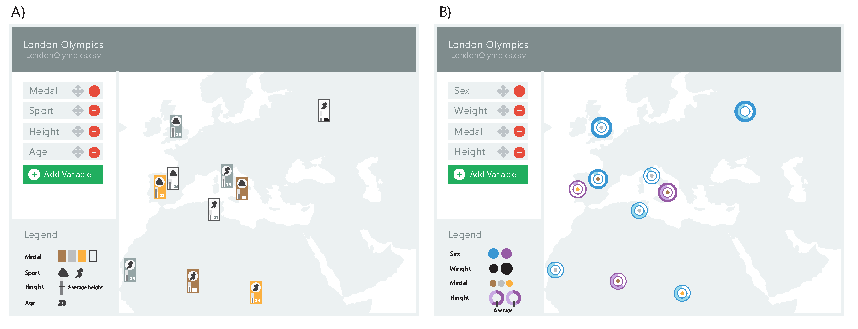
\includegraphics[width=\textwidth]{images/conclusion/glyph_exploration}
\caption{Glyph-based exploration of athletes competing in the London 2012 olympics.
A) Medal and sport are the most important variables for the task.
Less important visual variables such as height and age can be retrieved on closer inspection by zooming in.
B) Gender and weight are now the most important variables for the exploration task, resulting in a different glyph representation.}
\label{fig:glyph_exploration}
\end{figure}

An efficient encoding tool would present a path towards automatic glyph creation, extending on the \emph{GlyphMaker} work from twenty years ago by Ribarsky \etal \cite{ribarsky94}.
The decoding tool would help automatically validate a glyph design by measuring its effectiveness in terms of detecting how much information is available to a user at different resolutions, and what that information is.
Together, these would lay down a path for automatic glyph design (and validation), contributing towards a general-purpose glyph-based exploration library.

\item \textbf{Glyph-based data exploration} that would make glyph-based visualizations as easy to instantiate as parallel coordinates or scatter plot matrices.
Given a process for automated glyph creation exists, it should be possible to create task driven glyph-based visualizations that automatically change depending on the details a user felt most important in their analysis.
An example of how such a system may look is shown in Figures \ref{fig:glyph_exploration} A) and B) that show an interface whose glyphs change depending on the variables used and the ordering of their importance.

\item \textbf{Better quality measures} for glyph-based visualizations that extend on our quasi-Hamming distance metric introduced in Chapter \ref{chap:processes} to determine glyph distinguishability.
While glyph utility and memorability may not be suitable for assessment using computation, glyph interpretability could perhaps be measured using such an approach.
\end{enumerate}
